
\begin{frame}{Pourquoi un langage de programmation\,?}

SQL \alert{n'est pas} un langage de programmation
\begin{redbullet}

  \item SQL est un langage pensé pour permettre l'interrogation 
     d'une base de manière \alert{déclarative}, et non procédurale 
  
  \item Pas de variable, pas de boucle, pas de test
 
\end{redbullet}

\vfill

Pour écrire des applications, on utilise SQL associé à  un langage de programmation

\vfill
L'association\,:

\begin{redbullet}
  
  \item SQL pour les accès à la base
  \item Python, Java, PHP, C++, etc.  pour tout le reste

\end{redbullet}

\end{frame}

\begin{frame}{Deux architectures possibles}

Premier cas (à gauche)\,: les requêtes SQL sont intégrées à 
un \alert{programme client} et transmises au serveur de données.

\vfill

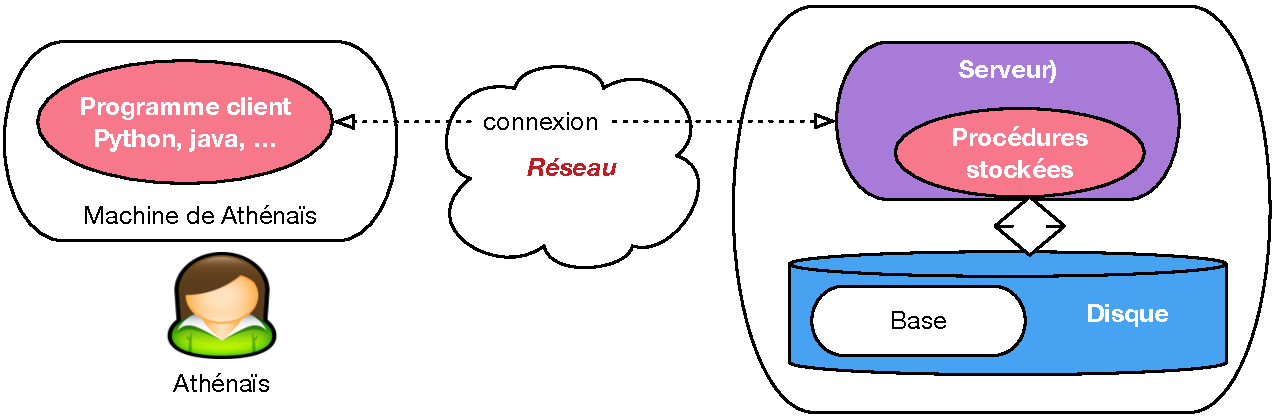
\includegraphics[width=10cm]{../figures-sql/architectures-prog}

\vfill

Second cas (à droite)\,:  requêtes SQL  intégrées au \alert{serveur} (procédures stockées)
moins d'échanges réseaux, plus de sécurité.
\end{frame}

\begin{frame}[fragile]{Illustration\,:  PL/SQL (Oracle)}

\begin{footnotesize}
\begin{minted}{sql}
    create procedure InsereLieu (p_lieu varchar) as 
      v_lieu_majuscules varchar(20);
      v_count integer;
    begin
      -- On met le paramètre en majuscules
      v_lieu_majuscules := upper(p_lieu);
      -- On verifie que le lieu n'existe pas 
      select count(*) into v_count 
      from Lieu where code = v_lieu_majuscules;
      -- Si on n'a rien trouvé: on insère
      if (v_count = 0) then
       insert into Lieu (code) values (v_lieu_majuscules);
     end if;
    end;
\end{minted}
\end{footnotesize}

\vfill 

Notez\,: les variables, la clause \sqlkw{into}, le test.

\end{frame}


\begin{frame}[fragile]{Second exemple, fonction et itérateur}

\begin{footnotesize}
\begin{minted}{sql}
create procedure MesActivités(v_code varchar) return varchar is
  -- Variable typée automatiquement
  v_activité Activité%rowtype; résultat = ""
  begin
      -- Boucle prenant toutes les activités du lieu
      for  v_activité in (select * from Activité
        where codeLogement = v_code)
      loop
          -- On concatène cette activité à la chaîne-résultat
          résultat := résultat || v_activité.codeActivité
      end loop;
     return résultat;
\end{minted}
\end{footnotesize}

\vfill
Notez\,: le type automatique de \texttt{v\_activité}, la boucle

\end{frame}

\begin{frame}[fragile]{Utilisation}

\begin{redbullet}

 \item Procédures\,: avec l'ordre \texttt{execute}, intégré à  un autre langage
 
   \begin{minted}{sql}
     execute insereLieu('Bretagne')
  \end{minted}
 
 \item Fonctions\,: dans une requête SQL
   \begin{minted}{sql}
      select nom, MesActivités(code) as activités 
      from Logement where code='ge';

nom      activités
-------  -----------------------------
Tabriz   Piscine, Ski
\end{minted}
 
\end{redbullet}

\end{frame}


%%%%%%%%%%%%%
\begin{frame}{À retenir}


Principales difficultés SQL/programmation\,:
\alert{typage} et \alert{conversion}

\vfill

\alert{Typage et conversion des nuplets}

\vfill

\begin{redbullet}
   \item Définir des variables du langage (Python, Java) correspondant aux types
       SQL
   \item Convertir le résultat d'une requête en variables du langage
\end{redbullet}

\vfill

\alert{Typage et conversion des tables}

\vfill

Ce sont des \alert{ensembles} (ou séquences si \sqlkw{order by}), on doit les parcourir avec des \alert{boucles}.

\end{frame}




